
\begin{table}
\caption{EMBERS system statistics}
 \centering
 \begin{tabular}{|l|l|l|l|l|}
 \hline
 Archived data     & 12.4 TB                  \\ \hline
 Archive size & ca. 3 billion messages   \\ \hline
 Data throughput   & 200-2000 messages/sec  \\ \hline
 Daily ingest & 15 GB \\ \hline
 System memory & 50 GB \\ \hline
 System core & 16 vCPUs \\ \hline
 System output & ca. 40 warnings/day \\ \hline
\end{tabular}
\label{tab:stats}
\end{table}



%\subsection{Linguistic Preprocessing}

As part of the general streaming architecture of the EMBERS system,
all textual input (e.g., tweets, news articles, blog postings) is
subjected to shallow linguistic processing prior to analysis.  Our
data set is multilingual, with Spanish, Portuguese and English
predominating in our data set. Commercial tools \footnote{BASIS
  Technology's Rossette Linguistic Platform \cite{}} are used for language
identification, tokenization, lematization and named entity
extraction. The lemmatized

Applying BASIS
technologies' Rosette Language Processing (RLP) tools, the language of
the text is identified, the natural language content is tokenized and
lemmatized and the named entities identified and classified. Date
expressions are normalized and deindexed (using the TIMEN
\cite{LlorensDGS12} package).  Finally, messages are geocoded with a
specification of the location (city, state, country), being talked
about in the message.  An example of this enrichment processing can be
seen in Fig.~\ref{fig:enrichment}.

\begin{figure}
    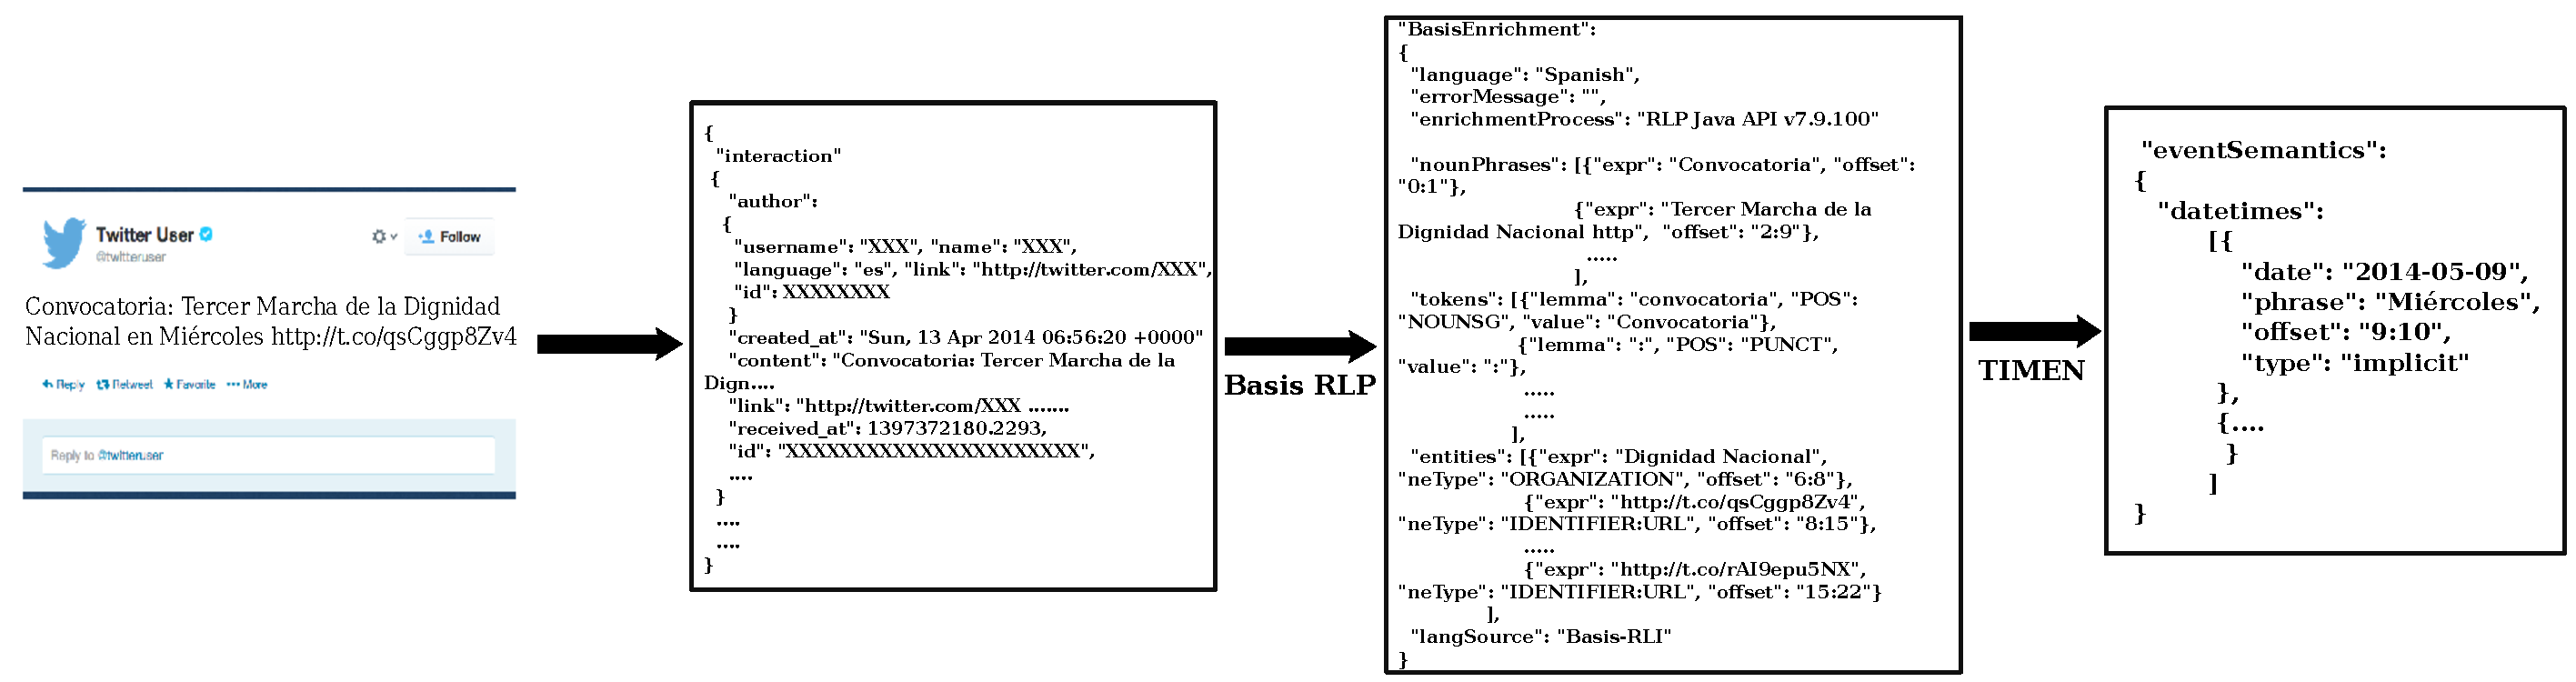
\includegraphics[width=0.5\textwidth]{enrichment}
    \caption{Message Enrichment}
    \label{fig:enrichment}
\end{figure}



%\begin{itemize}
%
%\item \textbf{TIMEN}: Date expressions are normalized and de-indexed using the TIMEN package -- {\em TIMEN: An Open Temporal Expression Normalisation Resource}.
%\end{itemize}
%

We make use of different geocoding methodologies for geo-coding news/blogs and twitter.

\subsection{Geo-Coding}

\subsubsection{News/Blogs}

\label{subsection:geocoding}
To extract the protest location from news articles, we use \emph{probabilistic soft logic} (PSL) \cite{broecheler:uai10} to build a model that performs robust, probabilistic inference given noisy signals. PSL takes a set of weighted, logic-like rules and converts them into a continuous probability distribution over the unknown truth values of logical facts. These truth values in PSL are relaxed into the $[0,1]$ interval. We use this mechanism to build a model that infers the semantic location of an article by weighing evidence coming from the Basis entity extractions and information in the World Gazatteer. 

The primary rules in the model encode the effect that Basis-extracted location strings that match to gazatteer aliases are indicators of the article's location, whether they be country, state, or city aliases. Each of these implications is conjuncted with an prior for ambiguous, overloaded aliases that is proportional to the population of the gazetteer location. For example, if the string ``Los Angeles'' appears in the article, it could refer to either Los Angeles, California, or Los \'{A}ngeles in Argentina or Chile. Given no other information, our model would infer a higher truth value for the article referring to Los Angeles, California, because it has a much higher population than the other options. 

\begin{align*}
    \begin{split}
    ENTITY(L, location) \softand REFERSTO(L, locID)\\
    \rightarrow PSLLOCATION(Article, locID)
\end{split}
\end{align*}


\begin{align*}
    \begin{split}
        ENTITY(C, location) \softand IsCountry(C)\\
    \rightarrow ArticleCountry(Article, C)
\end{split}
\end{align*}


\begin{align*}
    \begin{split}
        ENTITY(S, location) \softand IsState(S)\\
    \rightarrow ArticleCountry(Article, S)
\end{split}
\end{align*}

The secondary rules, which are given half the weight of the primary rules, perform the same mapping of extracted strings to gazetteer aliases, but for extracted persons and organizations. Strings describing persons and organizations often include location clues (e.g., ``mayor of Buenos Aires''), but intuition suggests the correlation between the article's location and these clues may be lower than with location strings. 

\begin{align*}
    \begin{split}
        ENTITY(O, organization) \softand REFERSTO(O, locID)\\
    \rightarrow PSLLOCATION(Article, locID)
\end{split}
\end{align*}


\begin{align*}
    \begin{split}
        ENTITY(O, organization) \softand IsCountry(O)\\
    \rightarrow ArticleCountry(Article, O)
\end{split}
\end{align*}


\begin{align*}
    \begin{split}
        ENTITY(O, organization) \softand IsState(O)\\
    \rightarrow ArticleCountry(Article, O)
\end{split}
\end{align*}
Finally, the model includes rules and constraints to require consistency between the different levels of geolocation, making the model place higher probability on states with its city contained in its state, which is contained in its country. As a post-processing step, we enforce this consistency explicitly by using the inferred city and its enclosing state and country, but adding these rules into the model makes the probabilistic inference prefer consistent predictions, enabling it to combine evidence at all levels.

\begin{align*}
    \begin{split}
        PSLLOCATION(Article, locID) \softand Country(locID, C)\\
    \rightarrow ArticleCountry(Article, C)
\end{split}
\end{align*}



\begin{align*}
    \begin{split}
        PSLLOCATION(Article, locID) \softand Admin1(locID, S)\\
    \rightarrow ArticleState(Article, S)
\end{split}
\end{align*}


\begin{figure*}
    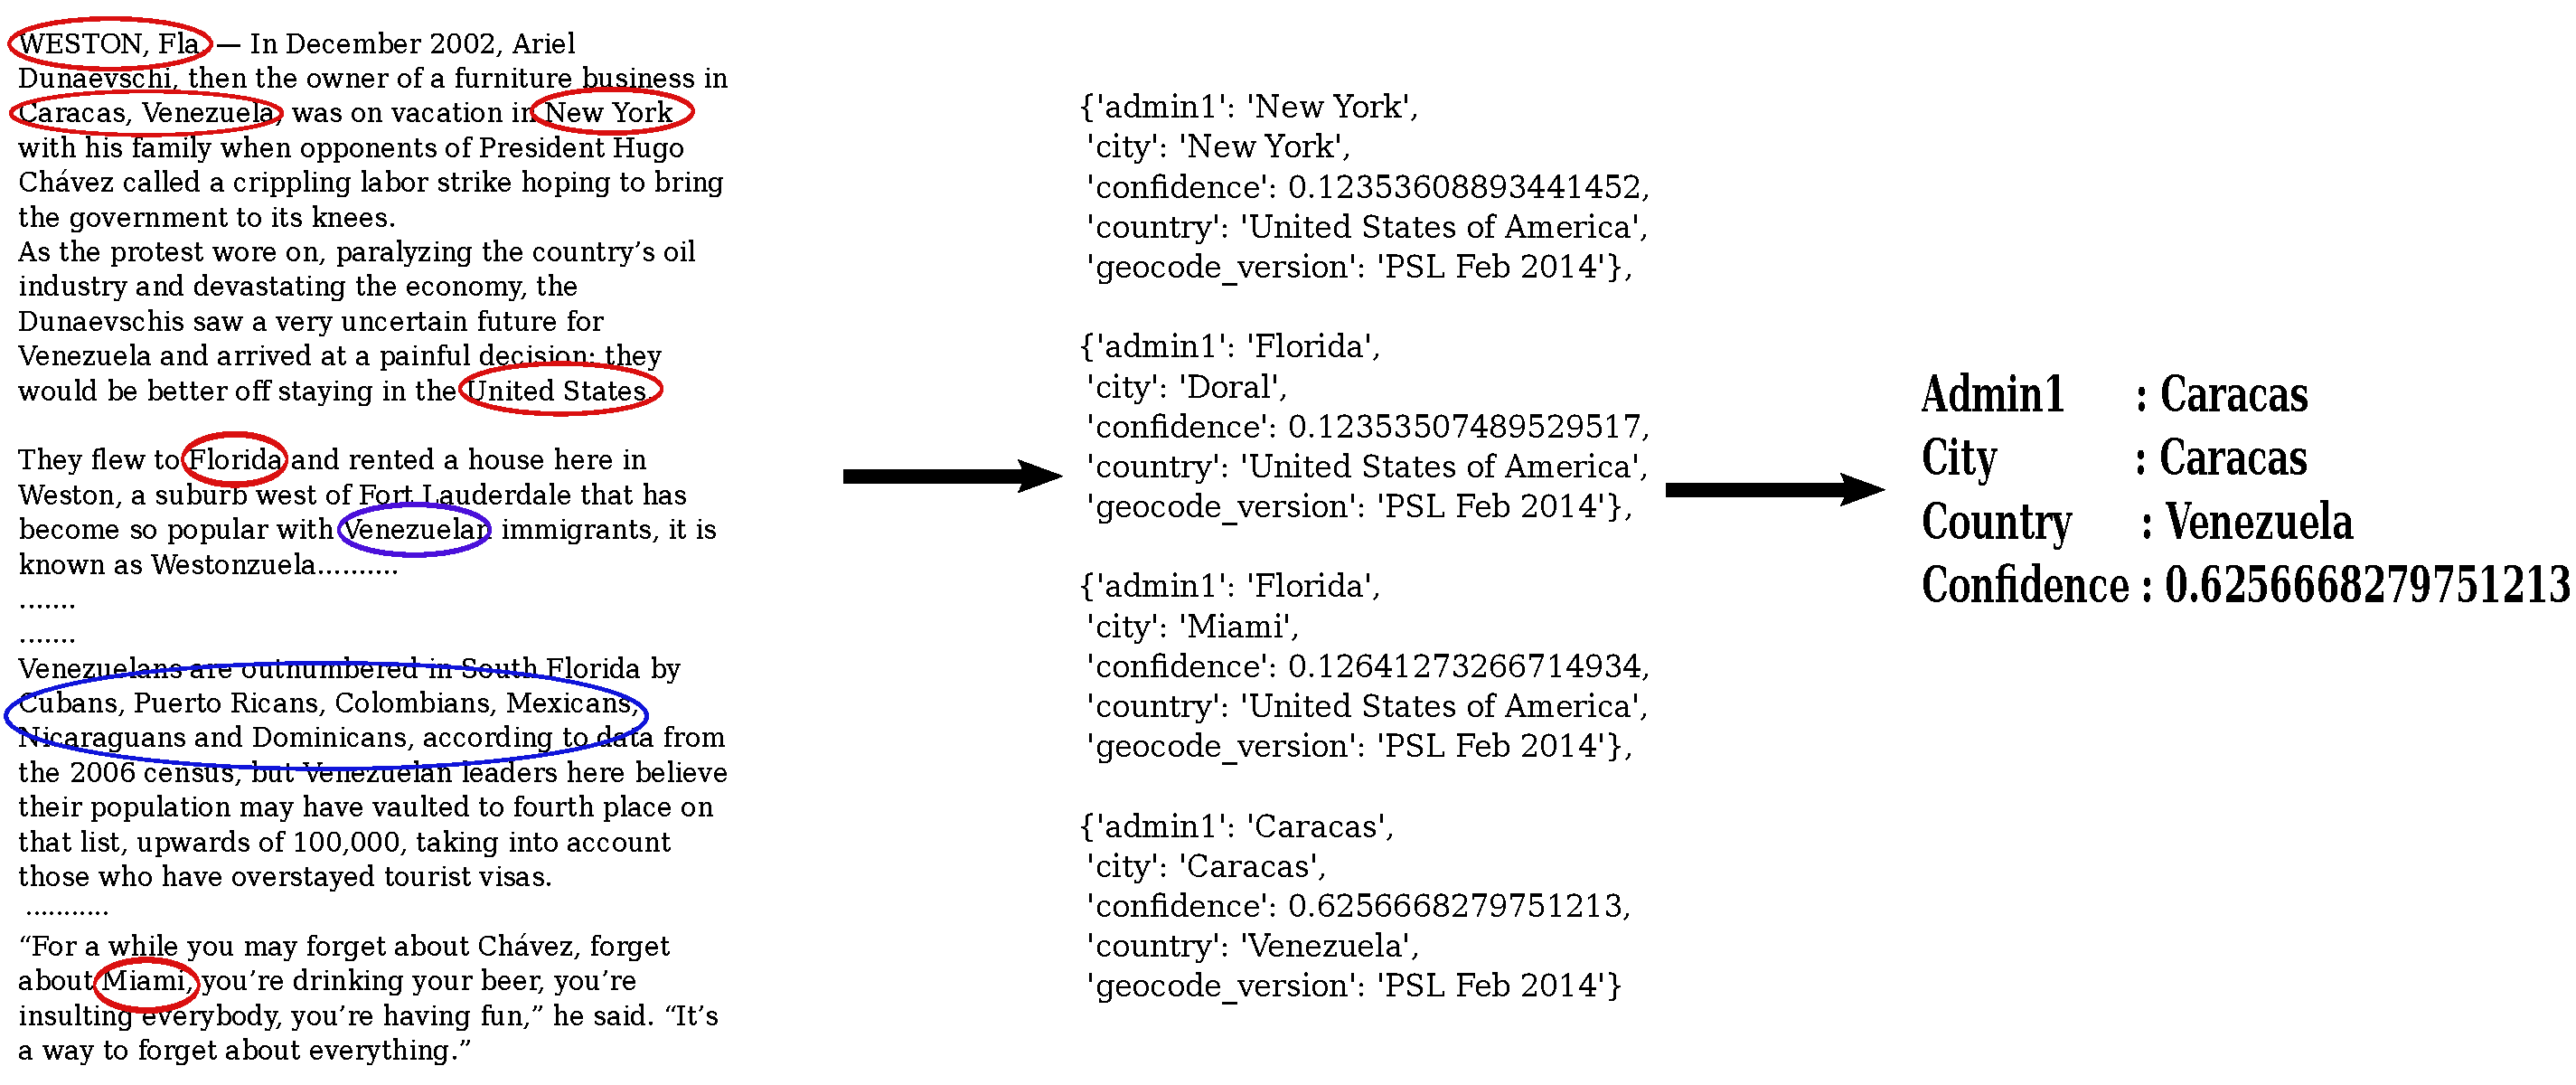
\includegraphics[width=\textwidth]{psl_pipeline}
    \caption{Red circles denote named entities identified as locations and blue denotes other types of entities. The article is reported from Weston Florida US and talks about the recent increase of venezuelan population in the US compared to other Latin American Nations like Cuba etc.}
    \label{fig:psl_example}
\end{figure*}
%%!TEX root = ../plannedprotest.tex

To extract the protest location from news articles, we use \emph{probabilistic soft logic} (PSL) \cite{broecheler:uai10;kimmig:probprog12} to build a model that performs robust, probabilistic inference given noisy signals. PSL takes a set of weighted, logic-like rules and converts them into a continuous probability distribution over the unknown truth values of logical facts. These truth values in PSL are relaxed into the $[0,1]$ interval. We use this mechanism to build a model that infers the semantic location of an article by weighing evidence coming from the Basis entity extractions and information in the World Gazatteer. 

The primary rules in the model encode the effect that Basis-extracted location strings that match to gazatteer aliases are indicators of the article's location, whether they be country, state, or city aliases. Each of these implications is conjuncted with an prior for ambiguous, overloaded aliases that is proportional to the population of the gazetteer location. For example, if the string ``Los Angeles'' appears in the article, it could refer to either Los Angeles, California, or Los \'{A}ngeles in Argentina or Chile. Given no other information, our model would infer a higher truth value for the article referring to Los Angeles, California, because it has a much higher population than the other options. 

The secondary rules, which are given half the weight of the primary rules, perform the same mapping of extracted strings to gazetteer aliases, but for extracted persons and organizations. Strings describing persons and organizations often include location clues (e.g., ``mayor of Buenos Aires''), but intuition suggests the correlation between the article's location and these clues may be lower than with location strings. 

Finally, the model includes rules and constraints to require consistency between the different levels of geolocation, making the model place higher probability on states with its city contained in its state, which is contained in its country. As a post-processing step, we enforce this consistency explicitly by using the inferred city and its enclosing state and country, but adding these rules into the model makes the probabilistic inference prefer consistent predictions, enabling it to combine evidence at all levels.

\iffalse Most news articles and blog posts mention multiple locations, e.g.,
the location of reporting, the location of the incident, and locations corresponding
to the hometown of the newspaper. We developed a probabilistic reasoning
engine using probabilistic soft logic (PSL)
to infer the most likely city, state and country which is the main geographic focus the article.The PSL geocoder combines various types of evidence, such as named entities
such as locations, persons, and organizations identified by RLP, as
well as common names and aliases and populations of known
locations. These diverse types of evidence are used in weighted rules
that prioritize their influence on the PSL model's location
prediction. For example, extracted location tokens are strong
indicators of the content location of an article, while organization
and person names containing location names are weaker but still
informative signals; the rules corresponding to these evidence types
are weighted accordingly.

The methodology is similar to {\em Web-a-where: Geo-Tagging Web Content}.
\fi 

\begin{figure}
    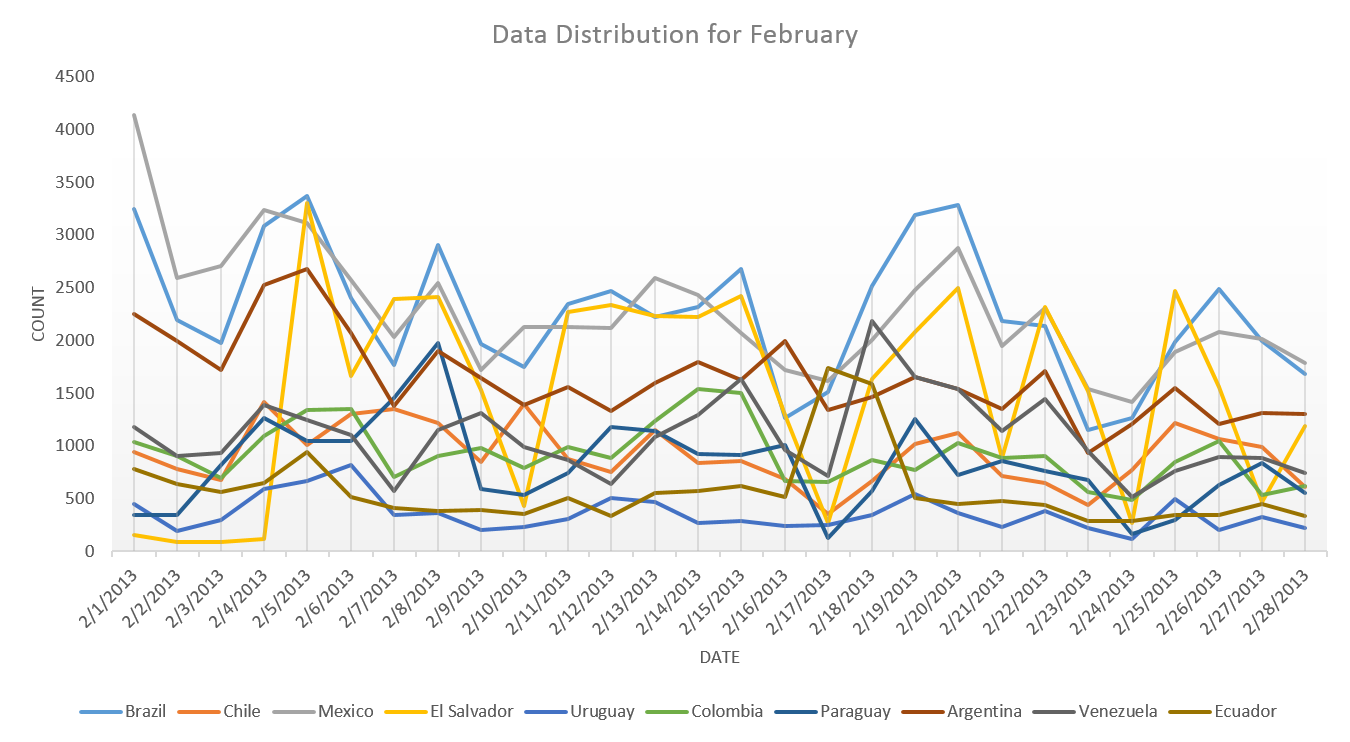
\includegraphics[width=0.5\textwidth]{rssdistribution}
    \caption{Rate of Arrival of News/Blogs}
    \label{fig:rssdistribution}
\end{figure}

\subsubsection{Twitter}
The Twitter\cite{twitter} geocoding is achieved by first
considering the most reliable but least available source,
viz. geotags, which give us exact geographic locations that can be
reverse geocoded into place names.  Second, we consider Twitter places
and use place names present in these fields to geocode the place names
into geographical coordinates.  Finally, we consider the text fields
contained in the user profile (location, description) as well as the
tweet text itself to find mentions of relevant locations which can
then be geocoded into geographical coordinates.

\subsubsection{Facebook}
We make use of only the facebook event data for our experiments. Facebook events that have a venue are only used. A venue of a facebook event generally contains a latitude, longitude, country, state, city, street, etc. Under cases where only latitude and longitude is given we do a reverse-geocoding by a KD-Tree lookup\cite{kd-tree} from the World Gazetteer to get the country, state, city information. 
